\documentclass{article} % For LaTeX2e
\usepackage{nips14submit_e,times}
\usepackage{amsmath}
\usepackage{amsthm}
\usepackage{amssymb}
\usepackage{mathtools}
\usepackage{hyperref}
\usepackage{url}
\usepackage{algorithm}
\usepackage[noend]{algpseudocode}
%\documentstyle[nips14submit_09,times,art10]{article} % For LaTeX 2.09

\usepackage{mathrsfs}
\usepackage{graphicx}
\usepackage{caption}
\usepackage{subcaption}

\def\eQb#1\eQe{\begin{eqnarray*}#1\end{eqnarray*}}
\def\eQnb#1\eQne{\begin{eqnarray}#1\end{eqnarray}}
\providecommand{\e}[1]{\ensuremath{\times 10^{#1}}}
\providecommand{\pb}[0]{\pagebreak}


\def\Qb#1\Qe{\begin{question}#1\end{question}}
\def\Sb#1\Se{\begin{solution}#1\end{solution}}

\newenvironment{claim}[1]{\par\noindent\underline{Claim:}\space#1}{}
\newtheoremstyle{quest}{\topsep}{\topsep}{}{}{\bfseries}{}{ }{\thmname{#1}\thmnote{ #3}.}
\theoremstyle{quest}
\newtheorem*{definition}{Definition}
\newtheorem*{theorem}{Theorem}
\newtheorem*{lemma}{Lemma}
\newtheorem*{question}{Question}
\newtheorem*{preposition}{Preposition}
\newtheorem*{exercise}{Exercise}
\newtheorem*{challengeproblem}{Challenge Problem}
\newtheorem*{solution}{Solution}
\newtheorem*{remark}{Remark}
\usepackage{verbatimbox}
\usepackage{listings}

\title{Real Variables: \\
Problem Set XI}


\author{
Youngduck Choi \\
Courant Institute of Mathematical Sciences \\
New York University \\
\texttt{yc1104@nyu.edu} \\
}


% The \author macro works with any number of authors. There are two commands
% used to separate the names and addresses of multiple authors: \And and \AND.
%
% Using \And between authors leaves it to \LaTeX{} to determine where to break
% the lines. Using \AND forces a linebreak at that point. So, if \LaTeX{}
% puts 3 of 4 authors names on the first line, and the last on the second
% line, try using \AND instead of \And before the third author name.

\newcommand{\fix}{\marginpar{FIX}}
\newcommand{\new}{\marginpar{NEW}}

\nipsfinalcopy % Uncomment for camera-ready version

\begin{document}


\maketitle

\begin{abstract}
This work contains solutions to the problem set 
XI of Real Variables 2015 at NYU.
\end{abstract}

\section{Solutions}

\begin{question}[Royden 17-6]
\hfill
\begin{figure}[h!]
  \centering
    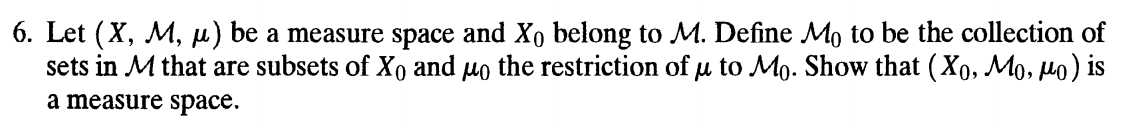
\includegraphics[width=1\textwidth]{rv-17-6.png}
\end{figure}
\end{question}
\begin{solution} 
We first show that $(X_0, \mathscr{M}_0)$ is a measurable space. To this
end, we must show that $\mathscr{M}_0$ is a $\sigma$-algebra of $X_0$.
As $\emptyset$ and $X_0$ belong to $\mathscr{M}$, are subsets of $X_0$,
it follows that $\emptyset$ and $X_0$ belong to $\mathscr{M}_0$. Let 
$\{A_n\}_{n=1}^{\infty}$ be a countable collections of sets in $\mathscr{M}_0$.
As $A_n \subseteq X_0$ for all $n$, we have $\bigcup_{n=1}^{\infty} A_n
\subseteq X_0$. Furthermore, as $\mathscr{M}$ is a $\sigma$-algebra, 
and $A_n \in \mathscr{M}$ for all $n$, we 
also have $\bigcup_{n=1}^{\infty} A_n \in \mathscr{M}$. Hence, it follows
that $\bigcup_{n=1}^{\infty} A_n \in \mathscr{M}_0$. Now, let $A$ be a 
set, belonging to $\mathscr{M}_0$. Then, 
as $X_0 \setminus A$ is a subset of
$X_0$, and $X_0$ and $A$ belong to $M$, which gives $X_0 \setminus A 
\in \mathscr{M}$, we have $X_0 \setminus A$ belongs to $\mathscr{M}_0$.
Hence, we have shown that $\mathscr{M}_0$ is a $\sigma$-algebra, and
$(X_0, \mathscr{M}_0)$ is a measurable space. Now, it remains to be
shown that the restricted map $\mu_0$ has the properties of a measure.
First, observe that $\emptyset \in \mathscr{M}_0$ and $\mu_0(\emptyset)
= \mu(\emptyset) = 0$. Now, let $\{A_n\}$ be a countable disjoint sets 
from $\mathscr{M}_0$. Since $A_n \in \mathscr{M}$ for all $n$,
by the countable additivity of $\mu$ and the fact that $\mathscr{M}_0$
is a $\sigma$-algebra,
it follows that 
\eQb
\sum_{n=1}^{\infty} \mu_0 (A_n) &=& \sum_{n=1}^{\infty} \mu(A_n) \\
&=& \mu(\bigcup_{n=1}^{\infty} A_n ) \\
&=& \mu_0(\bigcup_{n=1}^{\infty} A_n). \\
\eQe
Therefore, we have shown that $(X_0, \mathscr{M}_0, \mu_0)$ is
a measure space. \hfill $\qed$
 
\end{solution}

\newpage

\begin{question}[Royden 17-15]
\hfill
\begin{figure}[h!]
  \centering
    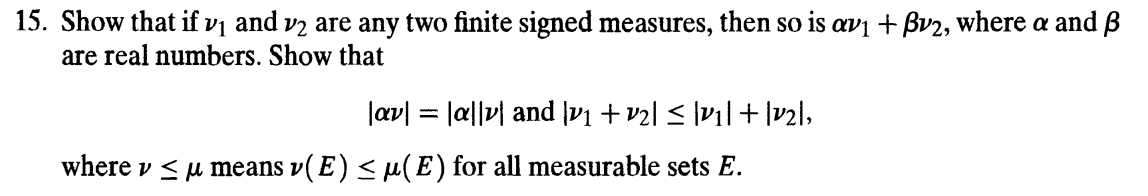
\includegraphics[width=1\textwidth]{rv-17-15.png}
\end{figure}
\end{question}
\begin{solution}
Let $(X,\mathscr{M})$ be a measurable space. 
Let $v_1$ and $v_2$ be two finite signed measures. Consider a 
set function $\alpha v_1 + \beta v_2$ on $\mathscr{M}$, for $\alpha , 
\beta \in \mathbb{R}$,
which is defined by
\eQb
\alpha v_1 + \beta v_2(E) &=& \alpha v_1(E) + \beta v_2(E) \\ 
\eQe
\end{solution}

\newpage

\begin{question}[Royden 17-17]
\hfill
\begin{figure}[h!]
  \centering
    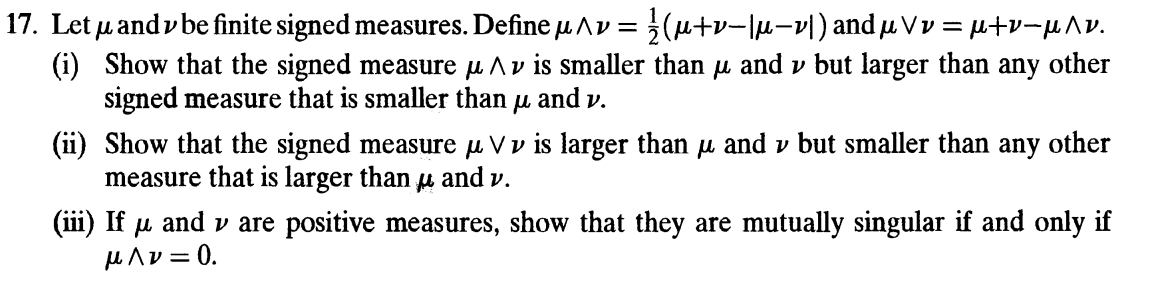
\includegraphics[width=1\textwidth]{rv-17-17.png}
\end{figure}
\end{question}
\begin{solution}
\end{solution}

\newpage

\begin{question}[Royden 18-50]
\hfill
\begin{figure}[h!]
  \centering
    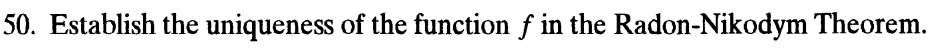
\includegraphics[width=1\textwidth]{rv-18-50.png}
\end{figure}
\end{question}
\begin{solution}
\end{solution}

\newpage

\begin{question}[Royden 18-54]
\hfill
\begin{figure}[h!]
  \centering
    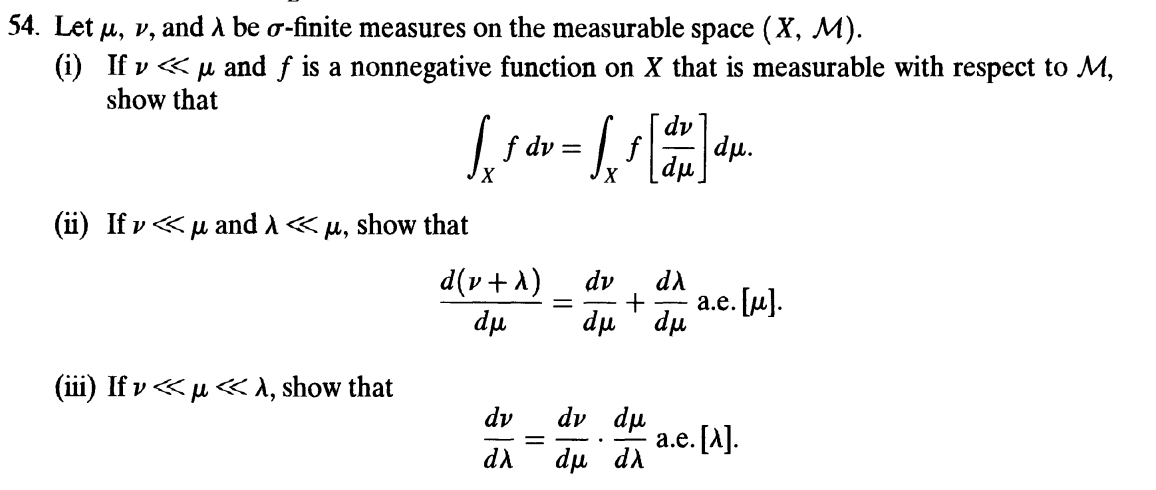
\includegraphics[width=1\textwidth]{rv-18-54.png}
\end{figure}
\end{question}
\begin{solution}
\end{solution}
\newpage

\begin{question}[Royden 18-55]
\hfill
\begin{figure}[h!]
  \centering
    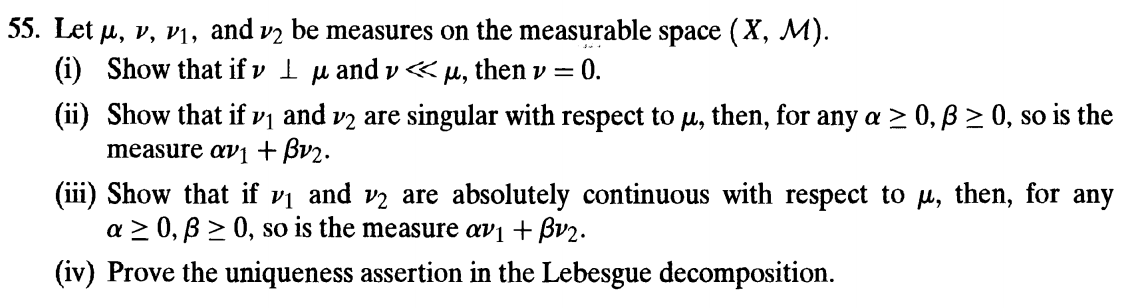
\includegraphics[width=1\textwidth]{rv-18-55.png}
\end{figure}
\end{question}
\begin{solution}
\end{solution}

\end{document}
